\chapter{Исследовательская часть}
В данном разделе приведены технические характеристики устройства, на котором проводилось измерение времени работы программного обеспечения, а также результаты замеров времени.

\section{Технические характеристики}
Характеристики используемого оборудования:
\begin{itemize}
    \item[$-$] Операционная система $-$ Windows 11 Home [9].
    \item[$-$] Память $-$ 16 Гб.
    \item[$-$] Процессор $-$ Intel(R) Core(TM) i5-10300H CPU @ 2.50ГГц [10].
    \item[$-$] Количество ядер $-$ 4 физических и 8 логических ядер.
\end{itemize}

\section{Замеры времени}
Для исследования зависимости времени отрисовки сцены от числа тел/лунок на сцене использовались одинаковые типы тел/лунок для каждой серии замеров. Время отрисовки замерялось на компьютере с указанными техническими характеристиками с помощью методов встроенного класса $Stopwatch$ [11]. Замеры времени проводились при добавлении различного количества тел (от 1 до 96) и лунок (от 1 до 19) и усреднялись для каждого набора экспериментов. Каждое значение получено путем взятия среднего из 5 измерений. Зависимости времени добавления тел и лунок от их количества представлены на рисунках \ref{fig:obj} $-$ \ref{fig:ind}.

% \begin{table}[h]
% 	\begin{center}
% 		\begin{threeparttable}
% 		\captionsetup{justification=raggedright,singlelinecheck=off}
% 		\caption{Время работы алгоритмов (в мс)}
% 		\label{tbl:time_measurements}
% 		\begin{tabular}{|c|r|r|r|r|}
% 			\hline
% 			Размер матрицы &  Классический & Виноград & Виноград (оптимизированный) \\
%             \hline
% 			1    & 0.12 & 0.34 & 0.30 \\
%             \hline
% 			2    & 0.55 & 0.52 & 0.50 \\ 
%             \hline
% 			4    & 1.05 & 0.62 & 0.52 \\ 
%             \hline
% 			8    & 1.56 & 1.56 & 1.50 \\ 
% 			\hline
% 			10    & 4.68 & 3.36 & 2.08 \\ 
% 			\hline
% 			20    & 28.60 & 4.16 & 19.76 \\ 
% 			\hline
% 			21    & 96.72 & 25.48 & 21.84 \\ 
% 			\hline
% 			32    & 299.00 & 92.04 & 76.96 \\ 
% 			\hline
% 			43    & 498.16 & 197.08 & 172.64 \\ 
% 			\hline
% 			54    & 890.24 & 417.56 & 359.32 \\ 
% 			\hline
% 			65    & 1628.64 & 777.40 & 670.28 \\ 
% 			\hline
%             76    & 2272.40 & 1161.16 & 991.12 \\ 
%             \hline
%             87    & 3104.16 & 1944.80 & 1682.20 \\ 
%             \hline
%             98   & 3307.20 & 2643.16 & 2276.04 \\ 
%             \hline
% 		\end{tabular}
% 		\end{threeparttable}
%     \end{center}
% \end{table}

\begin{figure}[H]
    \centering
    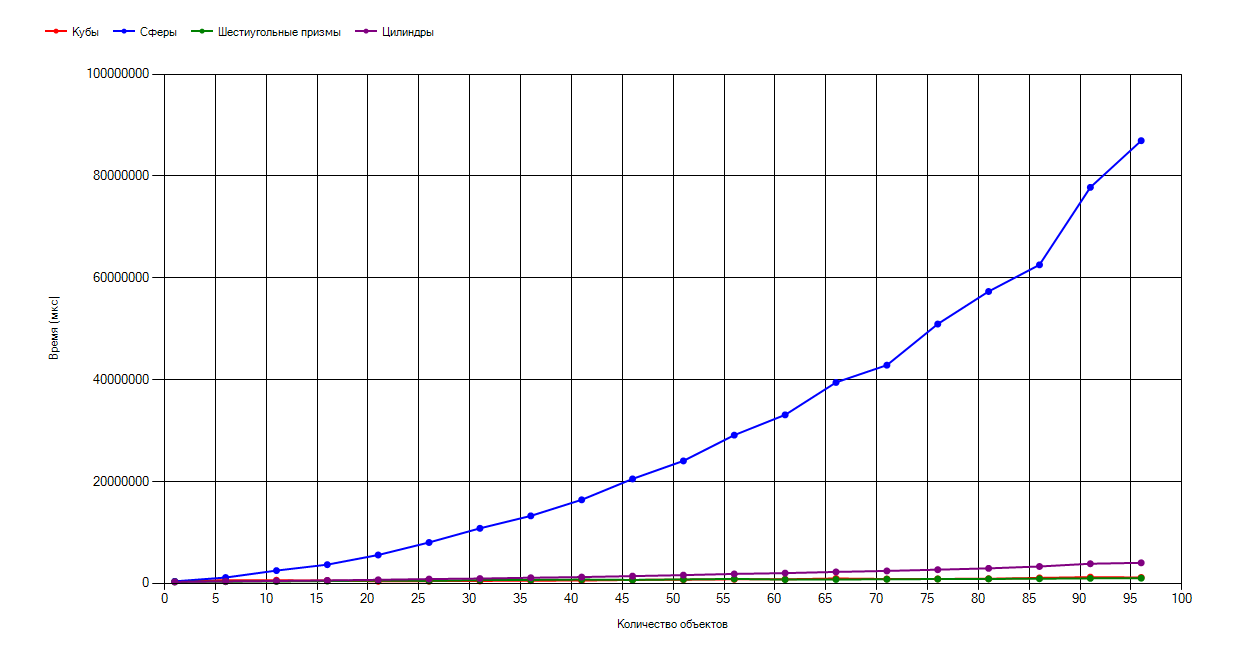
\includegraphics[width=1\linewidth]{img/graph_obj.png}
    \caption{График зависимости времени отрисовки от количества тел}
    \label{fig:obj}
\end{figure}

\begin{figure}[H]
    \centering
    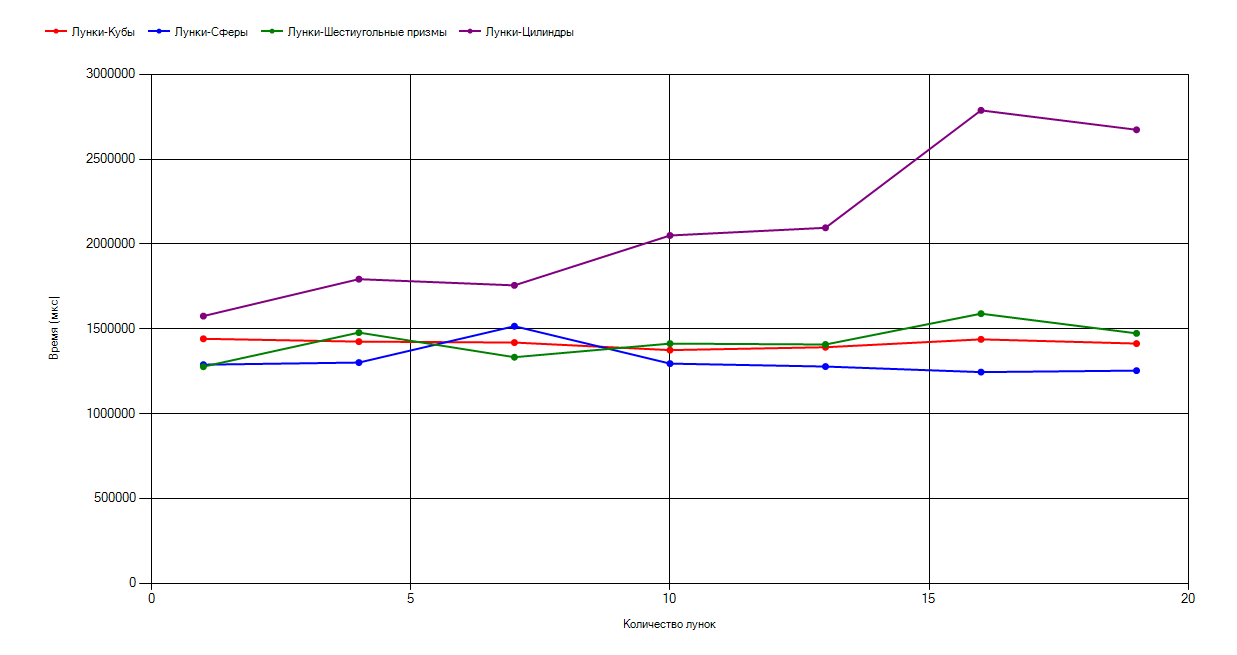
\includegraphics[width=1\linewidth]{img/graph_ind.png}
    \caption{График зависимости времени отрисовки от количества лунок}
    \label{fig:ind}
\end{figure}

В результате исследования было получено, что при увеличении количества тел, отрисовка каждой из них занимает больше времени. Наиболее значительное увеличение времени наблюдается при добавлении сфер, за которыми следуют цилиндры, шестигранные призмы и кубы. Это обусловлено большим количеством полигонов для представления каждой сферы и объемом вычислений, необходимых для их добавления и отображения. Зависимость времени отрисовки сцены от количества тел квадратична, так как алгоритм освещения с использованием алгоритма проверки затенения точки объектом имеет квадратичную сложность (см. схемы алгоритмов~\ref{fig:z}$-$~\ref{fig:shadow}).

Также было выявлено, что значительное увеличение времени наблюдается при добавлении цилиндрических и сферических лунок, что обусловлено более сложной геометрией этих форм и необходимостью выполнения дополнительных вычислений для их корректного отображения. Лунки для кубов и шестигранных призм демонстрируют стабильное увеличение времени при добавлении, что свидетельствует о меньшей сложности их обработки по сравнению с цилиндрическими или сферическими.

\textbf{ВЫВОД}

В данном разделе приведены результаты работы программного обеспечения и результаты исследования.
Результаты исследования совпали с ожидаемыми, так как время отрисовки сцены прямо пропорционально количеству объектов и лунок на сцене и сложности математических расчетов.
\clearpage